\documentclass[12pt,a4paper]{article}
\usepackage{amsmath}
\usepackage{graphicx}
\usepackage{geometry}
\usepackage{float}
\geometry{left=2cm,right=2cm,top=2.5cm,bottom=2.5cm}

\title{\textbf{Multi-Branch Kinematic Analysis Report \\ (Separate Branch Visualization)}}
\author{Automated Generation System}
\date{\today}

\begin{document}
\maketitle

\section{Assembly Modes (Branches) Overview}
Due to the highly nonlinear nature of the closed-loop constraints, spatial 7R mechanisms typically exhibit multiple assembly modes (kinematic branches) for the same driving input. Our algorithm successfully identified \textbf{4} distinct branches by applying diverse initial perturbations at $q_1 = 0^\circ$.

\section{Matrix Calculation (Branch A Example at $q_1 = 0^\circ$)}
We extract the matrices for the first identified branch (Branch A). The full joint configuration is:
\begin{equation}
    \mathbf{q}_A = \begin{bmatrix} 0.0000 \\ -0.0231 \\ -0.0002 \\ 0.0462 \\ 0.0003 \\ 0.0231 \\ -0.0005 \end{bmatrix}
\end{equation}

The passive Jacobian $J_p \in \mathbb{R}^{6 \times 6}$ (removing column 1):
\begin{equation}
    \resizebox{0.85\textwidth}{!}{$ J_p = \begin{bmatrix}
  0.000 & 0.000 & 2.499 & 0.058 & -2.500 & -0.000 \\
  -1.000 & -0.000 & 2.999 & 0.000 & 1.998 & -0.000 \\
  0.000 & -3.000 & -0.058 & -0.500 & -0.058 & -2.000 \\
  0.000 & 0.000 & -0.023 & 0.000 & -0.023 & -0.001 \\
  0.000 & -1.000 & -0.000 & -1.000 & -0.000 & 1.000 \\
  1.000 & 0.000 & -1.000 & -0.000 & 1.000 & -0.000
\end{bmatrix} $}
\end{equation}

Singular Values matrix $\Sigma$:
\begin{equation}
    \resizebox{0.85\textwidth}{!}{$ \Sigma = \begin{bmatrix}
  4.178 & 0.000 & 0.000 & 0.000 & 0.000 & 0.000 \\
  0.000 & 3.671 & 0.000 & 0.000 & 0.000 & 0.000 \\
  0.000 & 0.000 & 3.352 & 0.000 & 0.000 & 0.000 \\
  0.000 & 0.000 & 0.000 & 1.669 & 0.000 & 0.000 \\
  0.000 & 0.000 & 0.000 & 0.000 & 0.892 & 0.000 \\
  0.000 & 0.000 & 0.000 & 0.000 & 0.000 & 0.000
\end{bmatrix} $}
\end{equation}

\clearpage
\section{Kinematic \& Singularity Plots for Each Branch}
The continuous kinematic mappings and corresponding Singular Value Decomposition (SVD) evolutions for each identified branch are plotted below.

\begin{figure}[H]
    \centering
    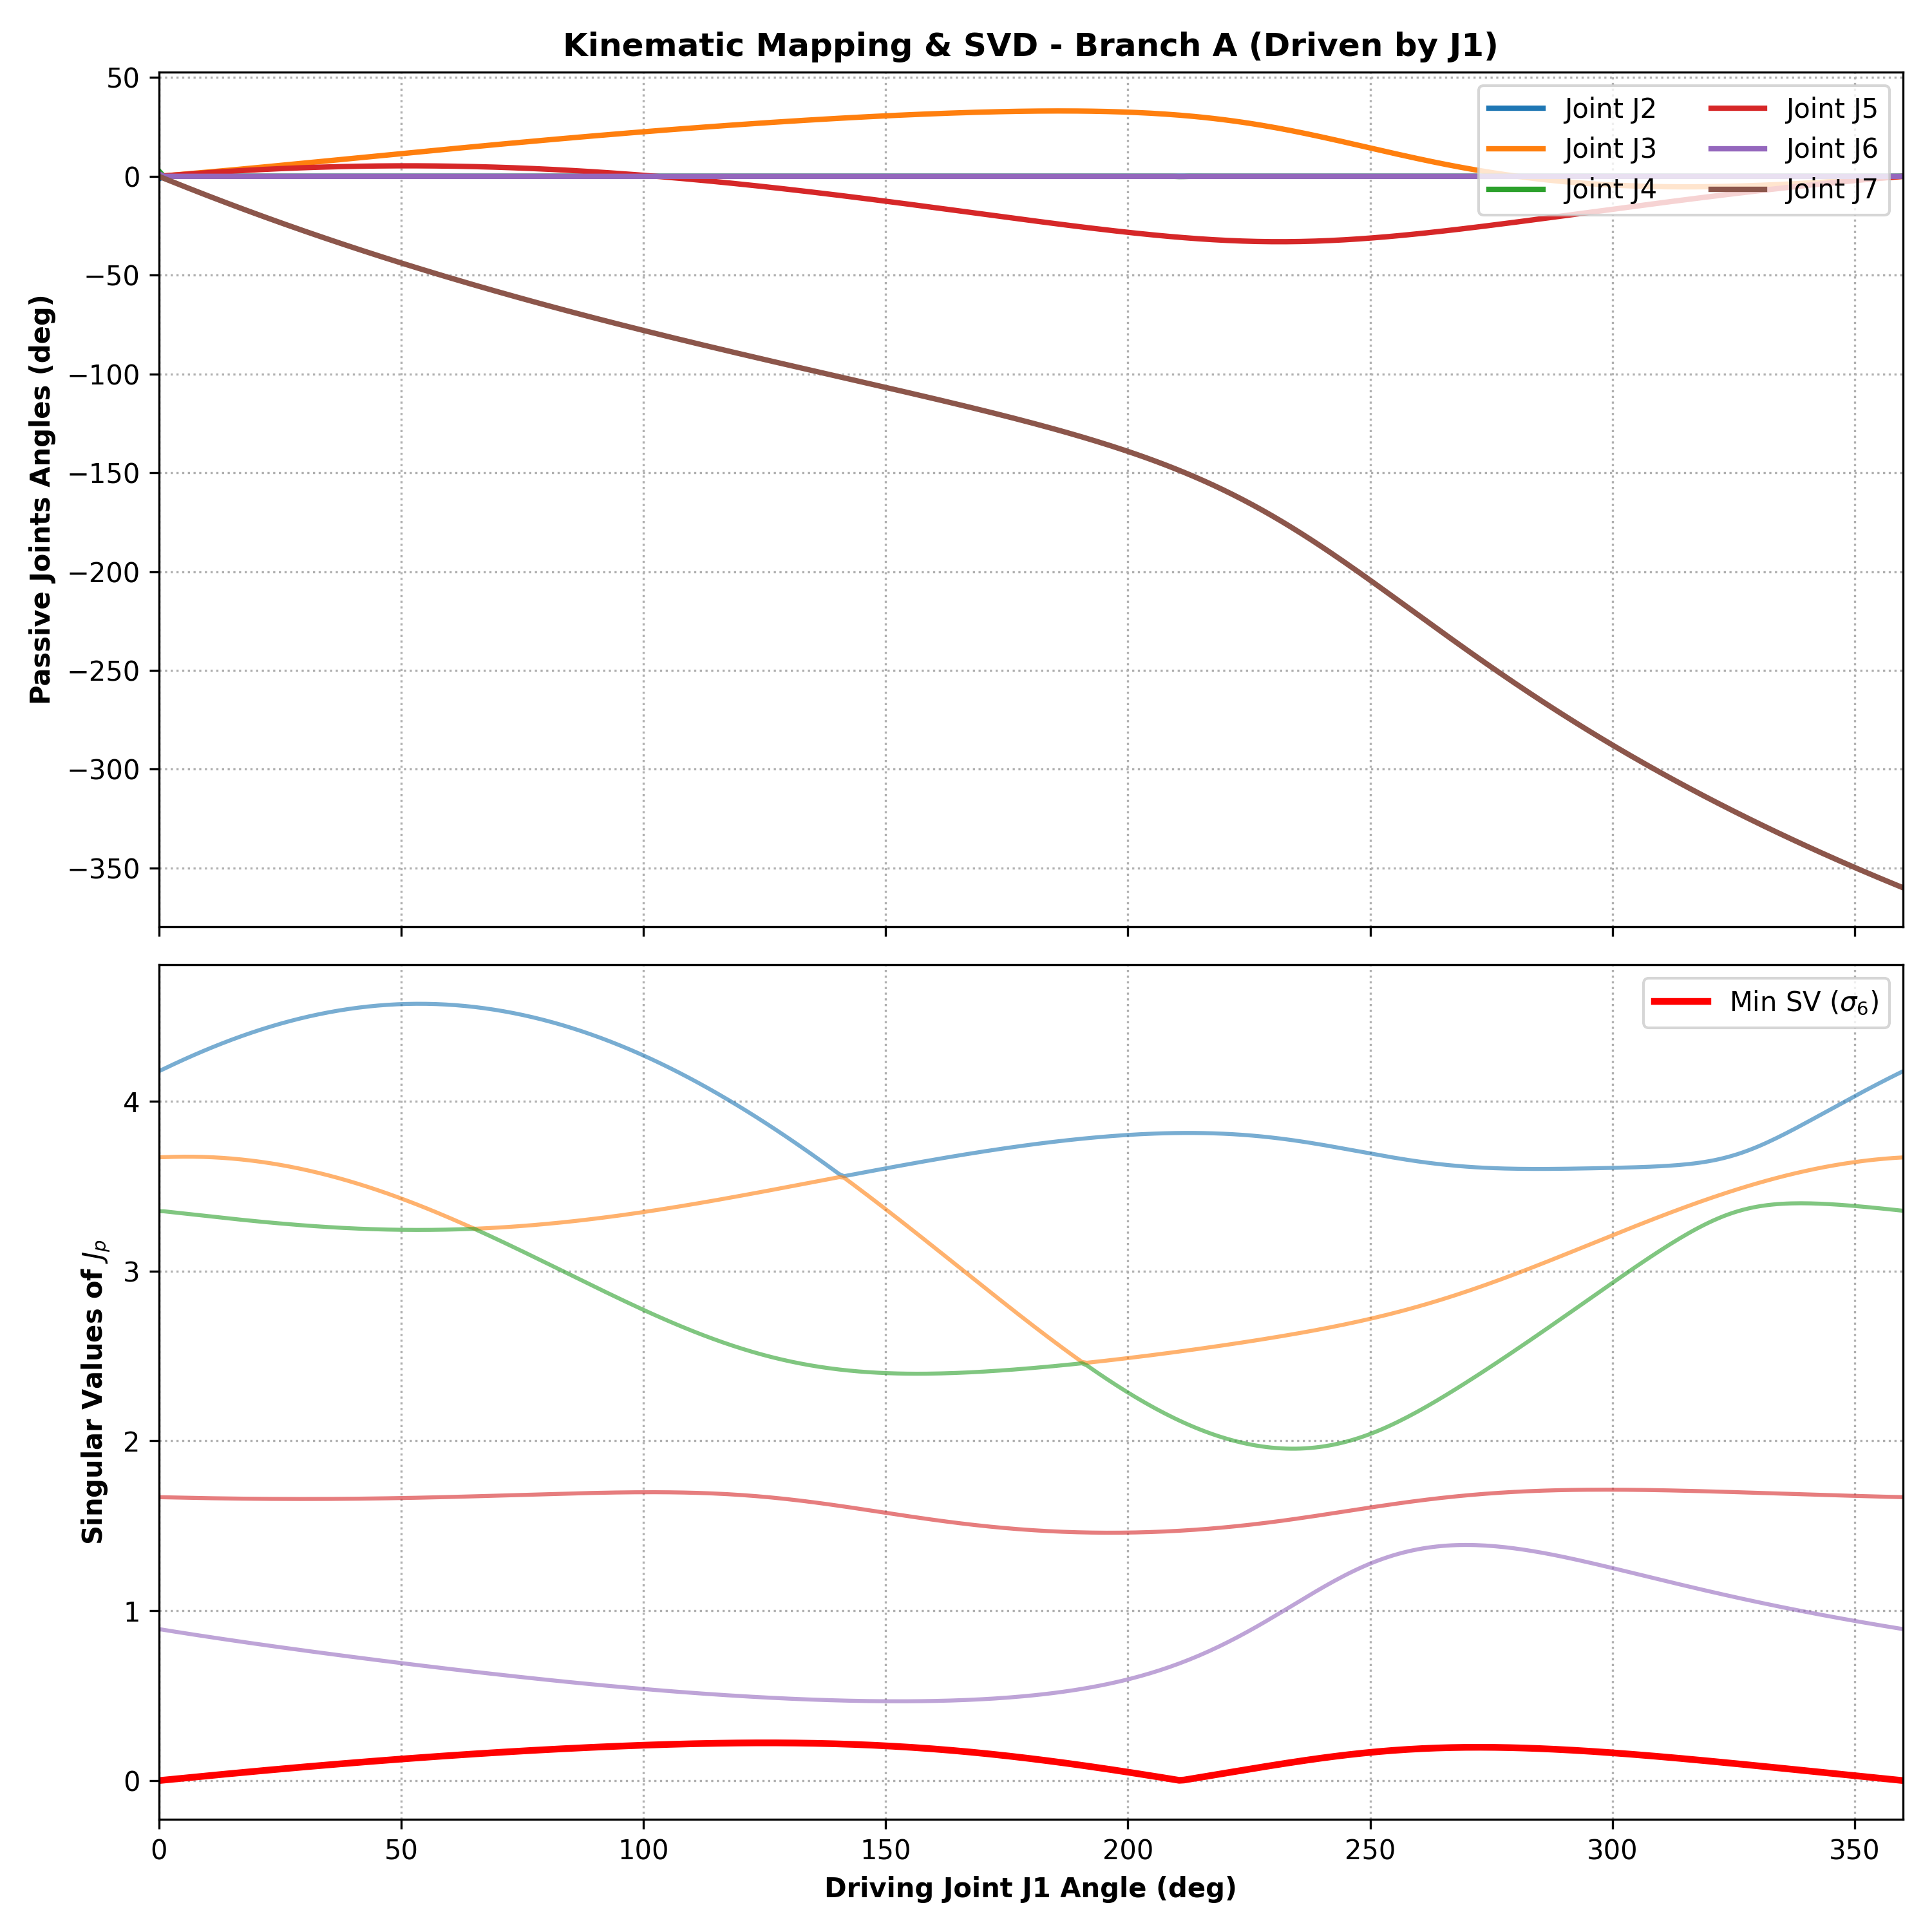
\includegraphics[width=0.9\textwidth]{j1_branch_A_plot.png}
    \caption{Kinematic mapping and singular value evolution for \textbf{Branch A} (Driven by $J_1$).}
\end{figure}

\begin{figure}[H]
    \centering
    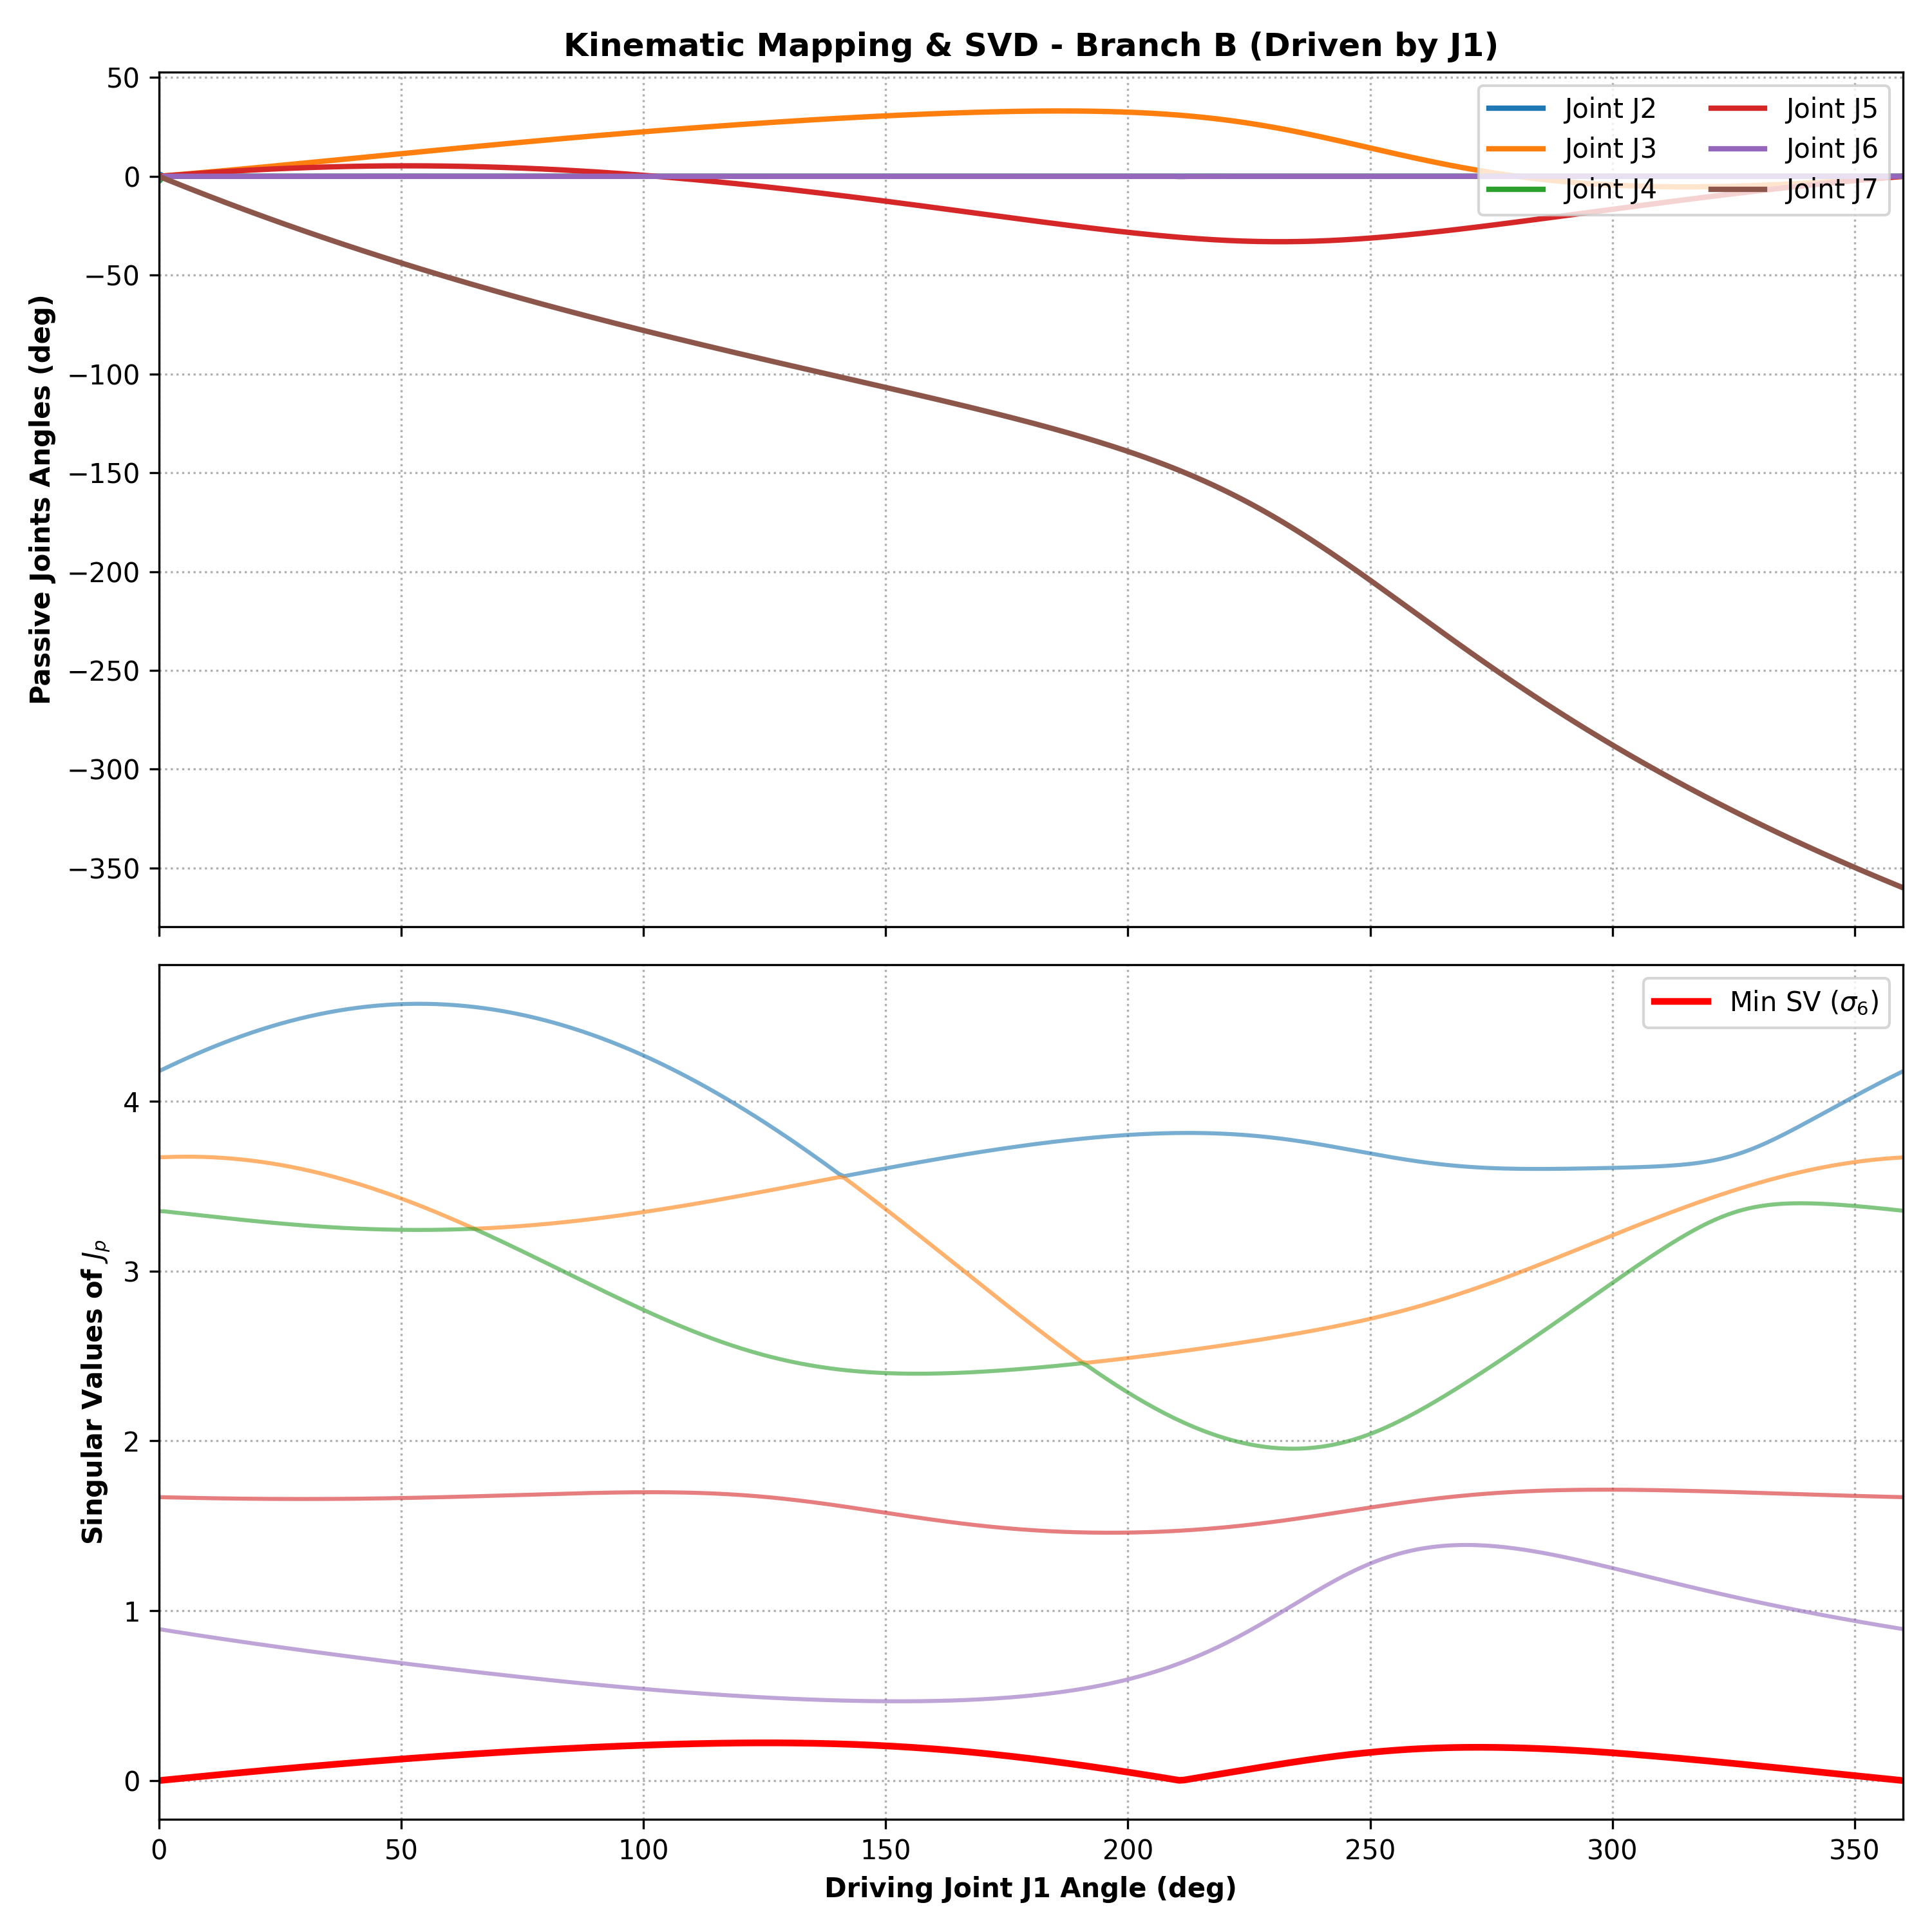
\includegraphics[width=0.9\textwidth]{j1_branch_B_plot.png}
    \caption{Kinematic mapping and singular value evolution for \textbf{Branch B} (Driven by $J_1$).}
\end{figure}

\begin{figure}[H]
    \centering
    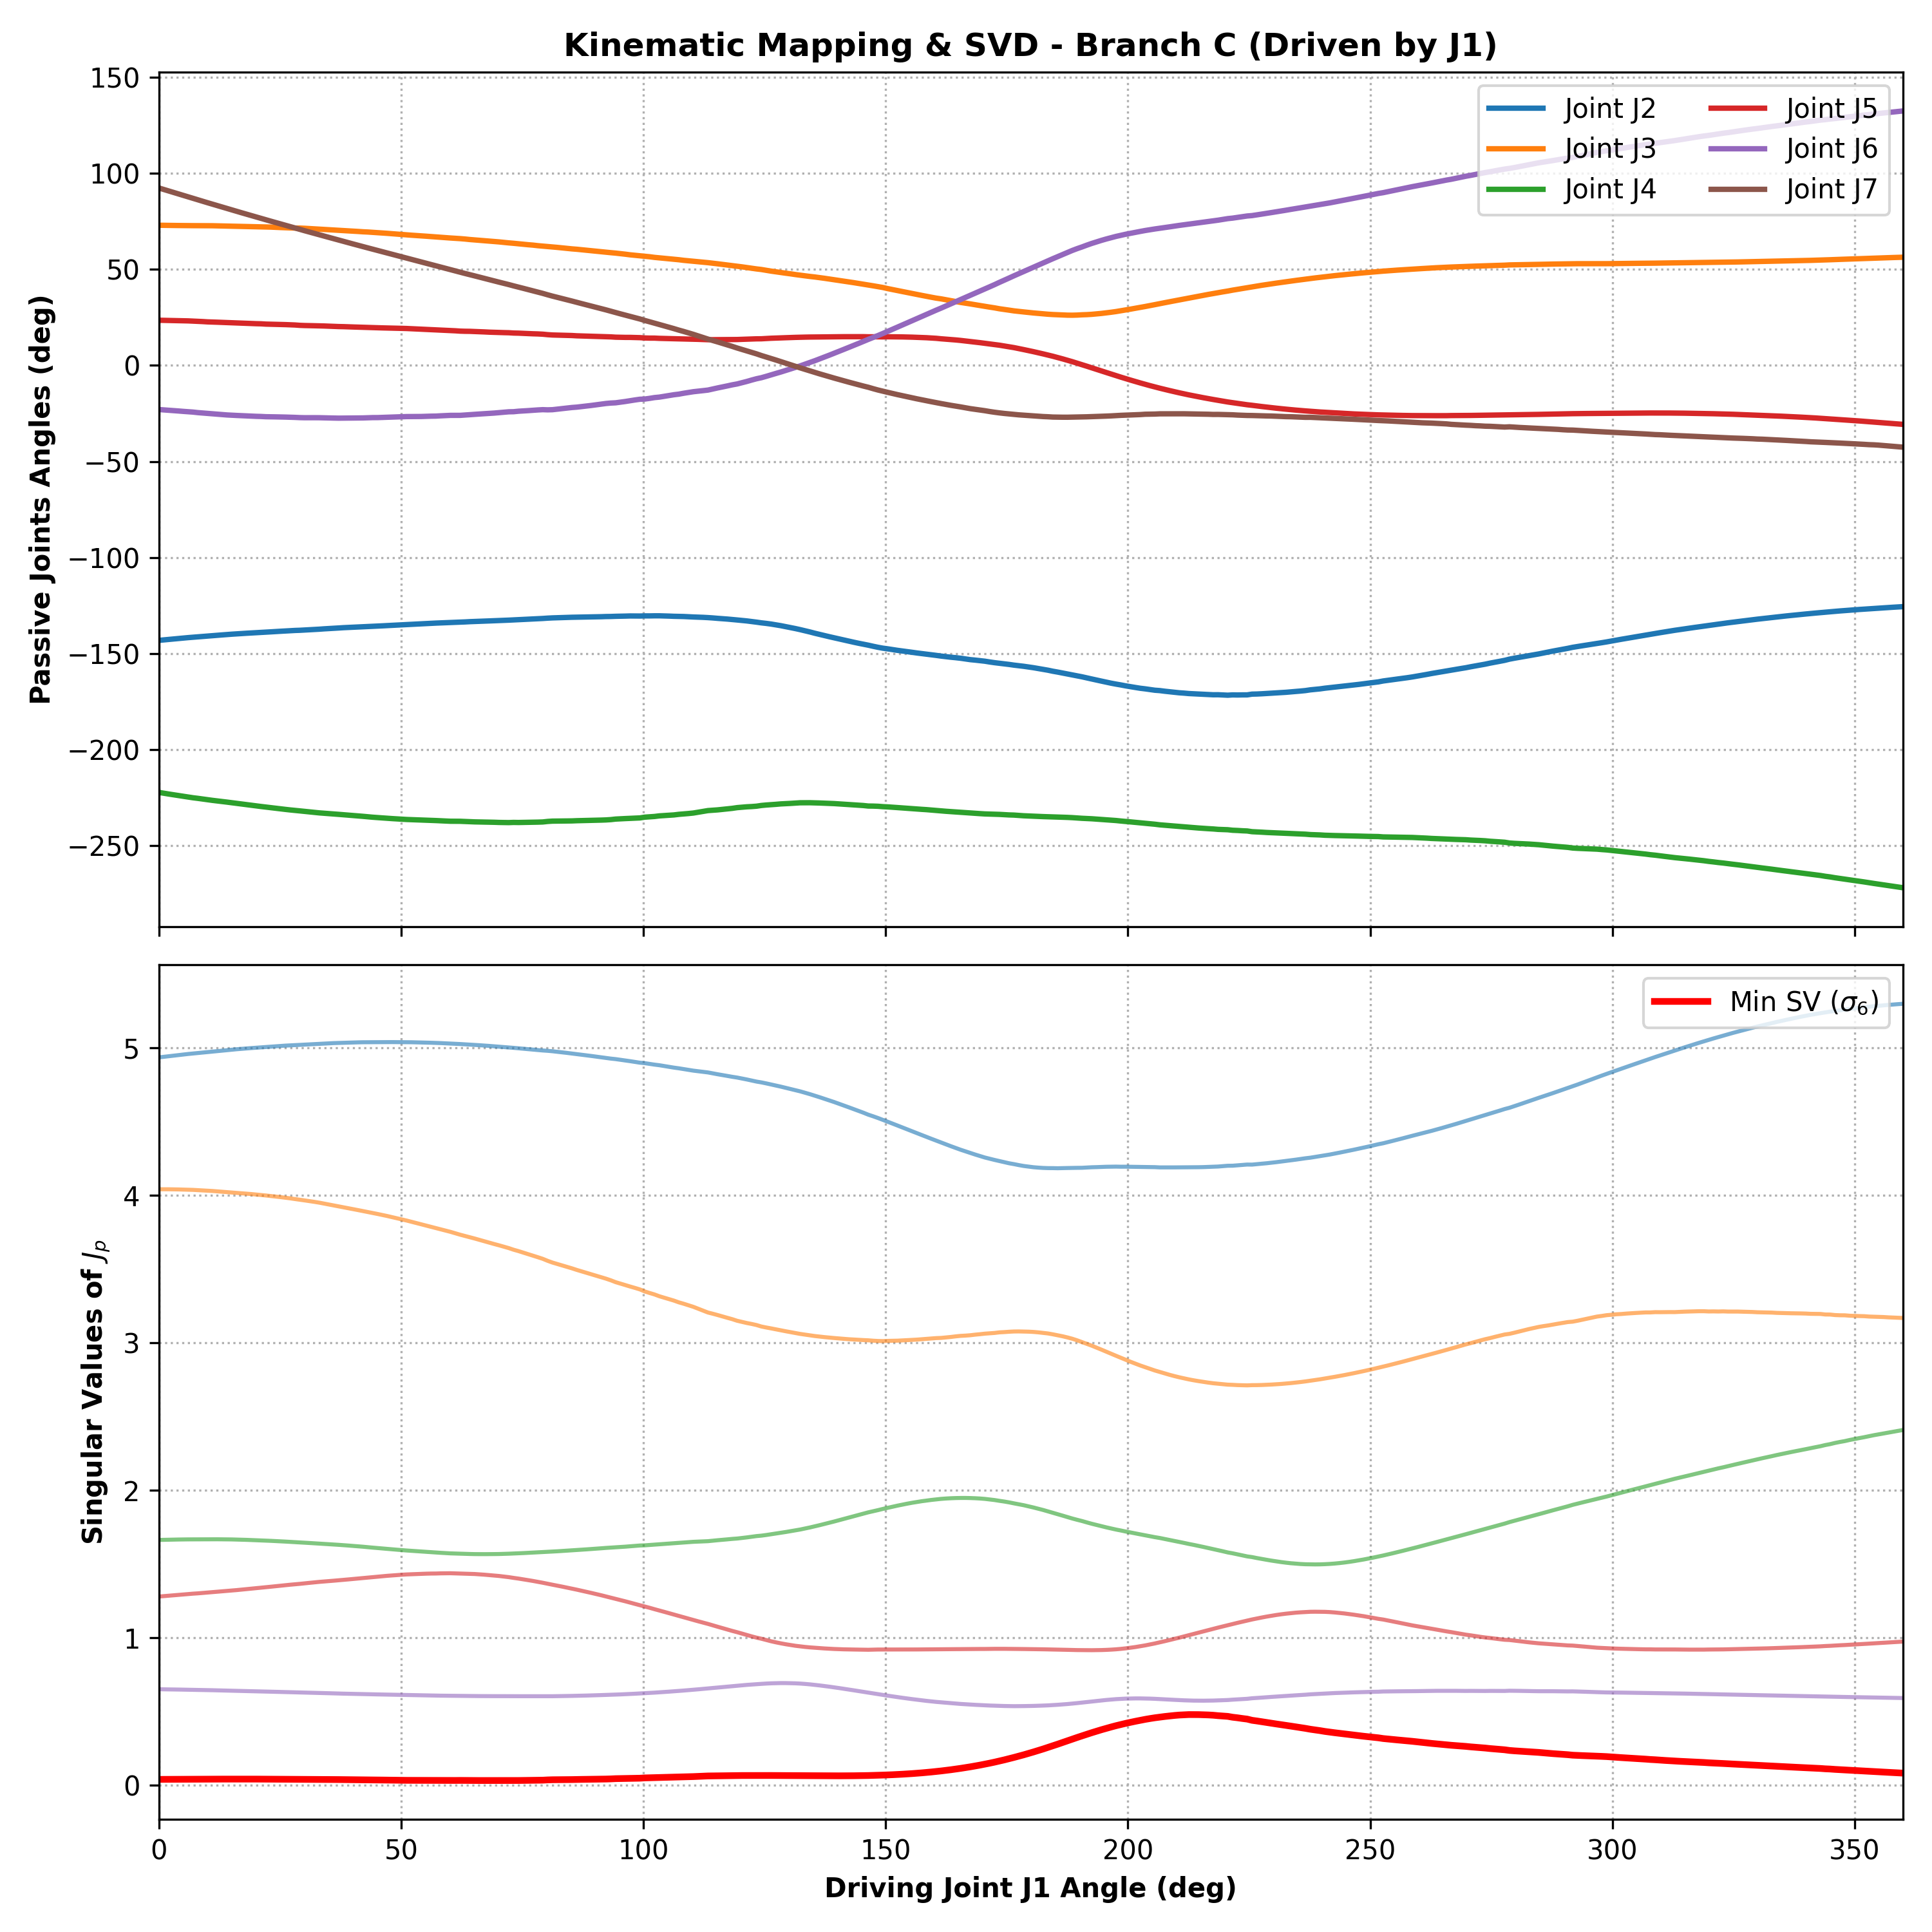
\includegraphics[width=0.9\textwidth]{j1_branch_C_plot.png}
    \caption{Kinematic mapping and singular value evolution for \textbf{Branch C} (Driven by $J_1$).}
\end{figure}

\begin{figure}[H]
    \centering
    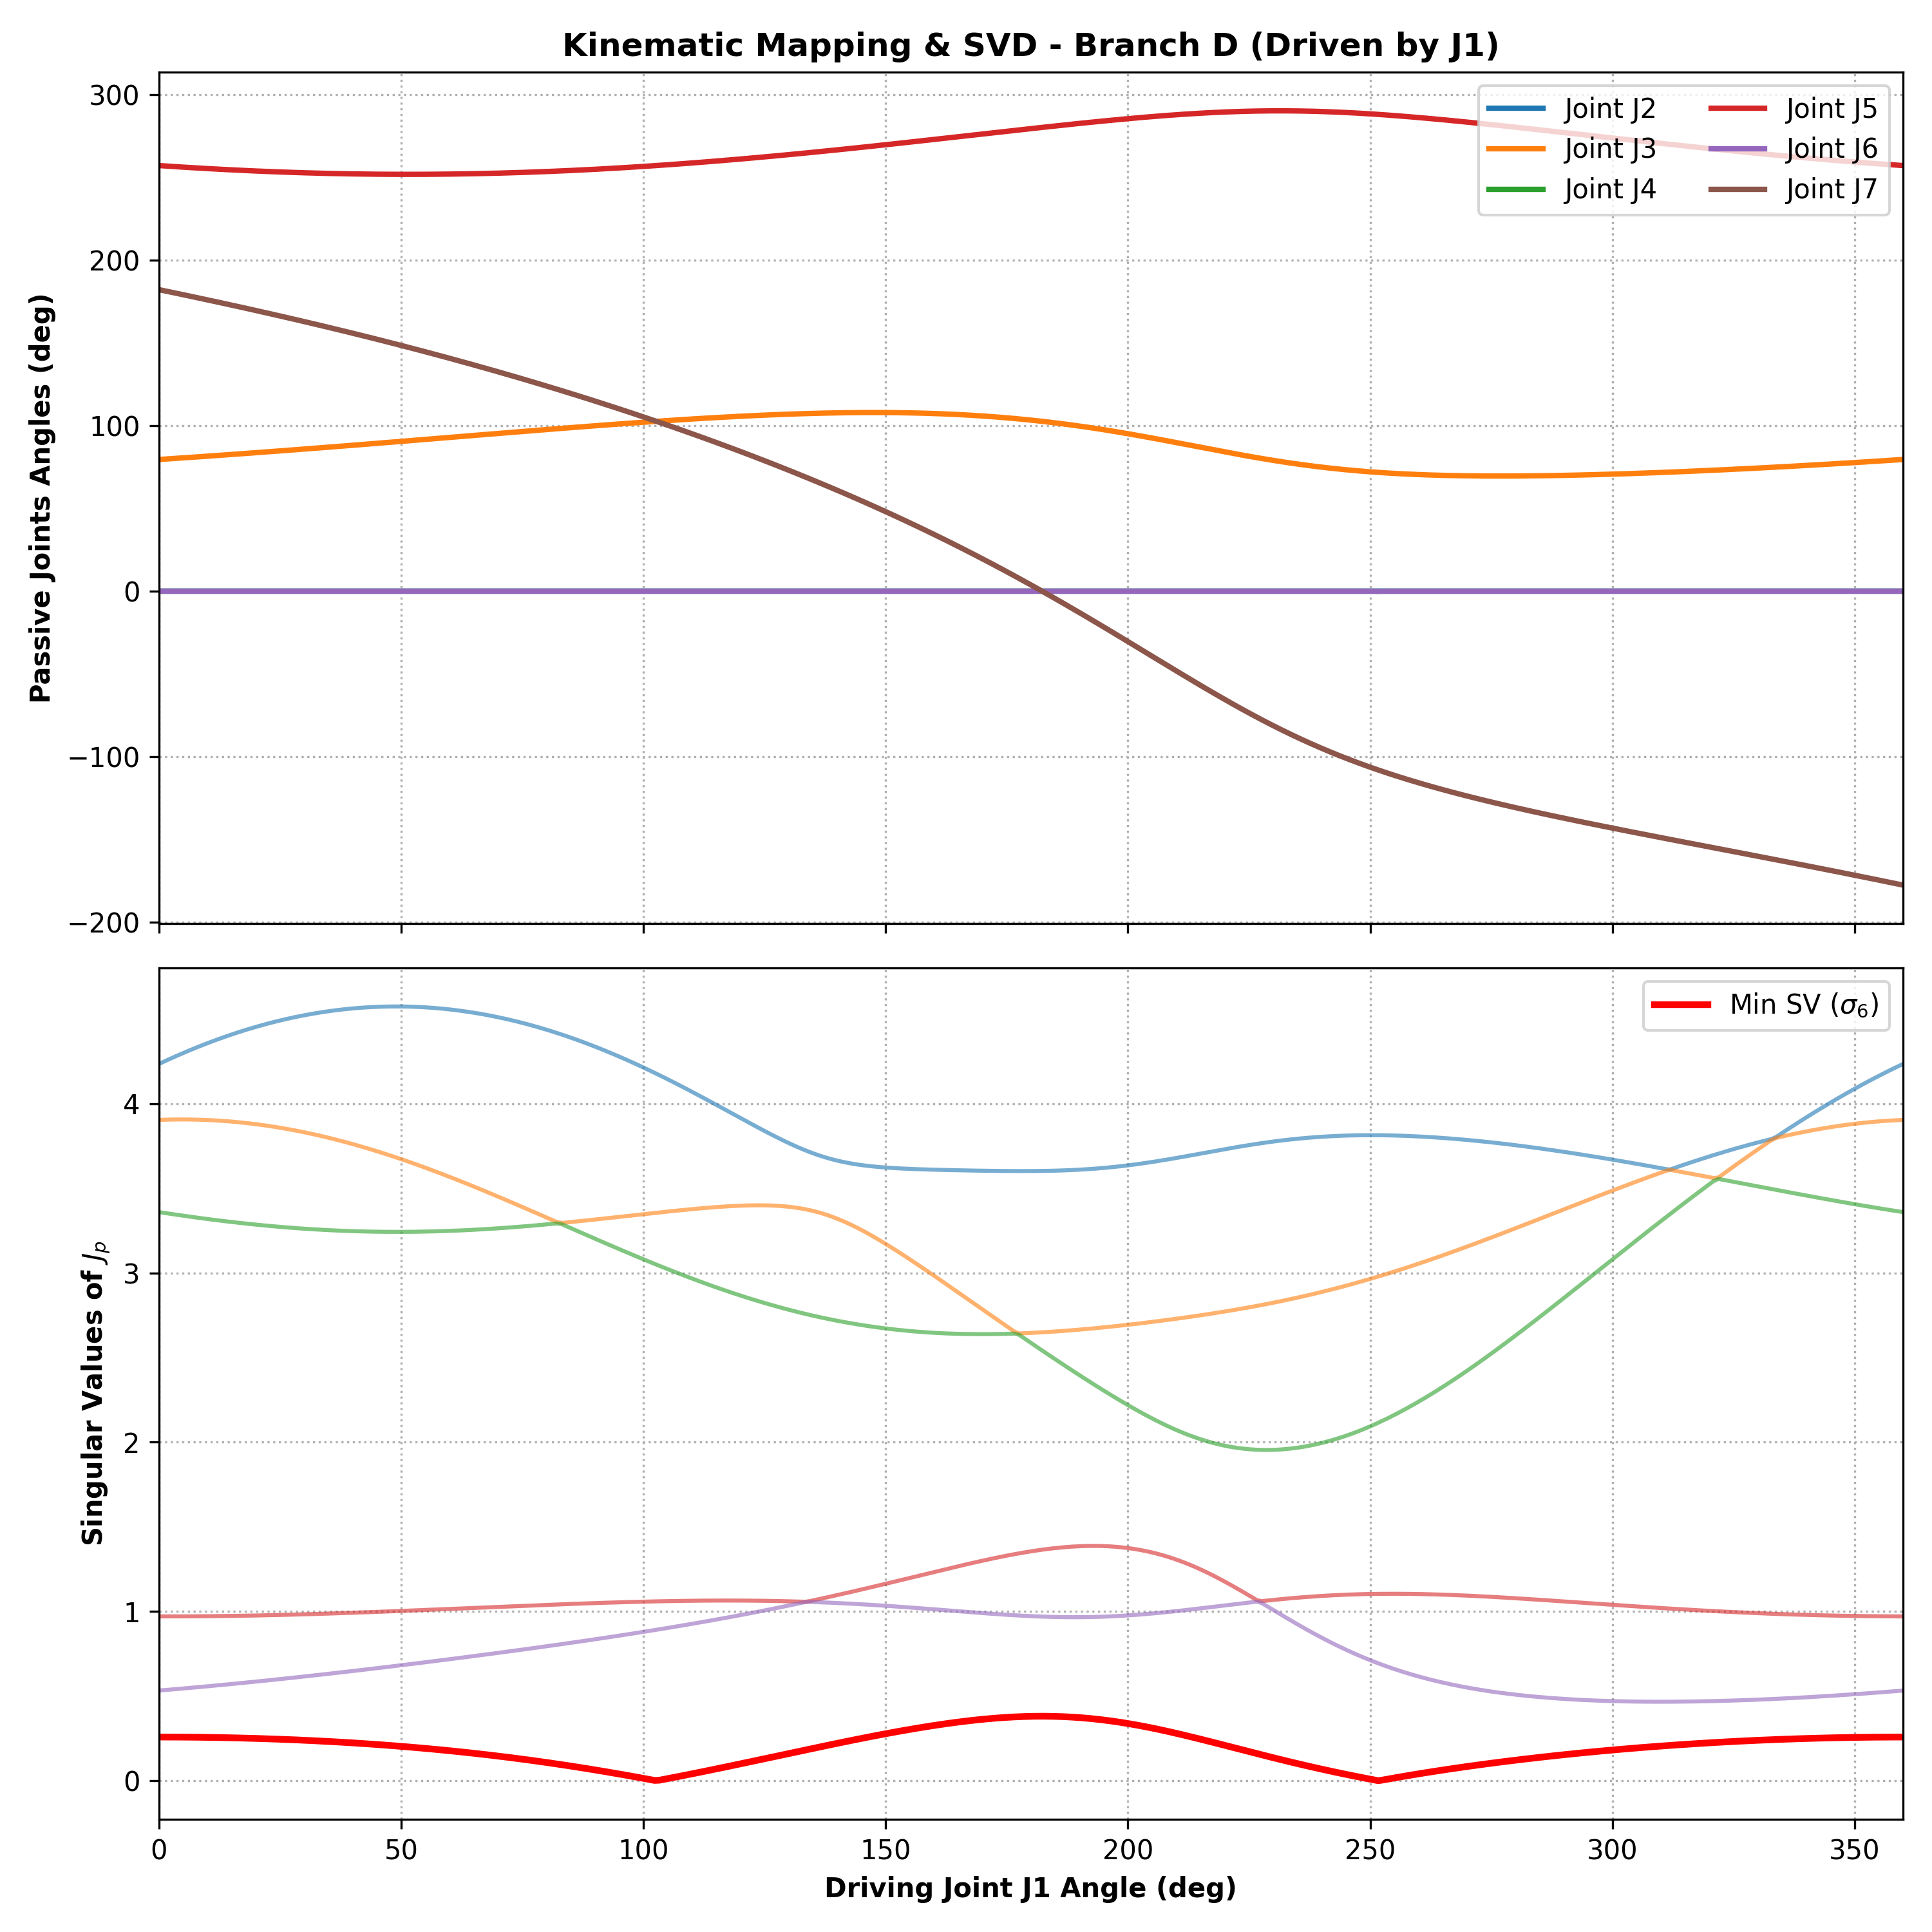
\includegraphics[width=0.9\textwidth]{j1_branch_D_plot.png}
    \caption{Kinematic mapping and singular value evolution for \textbf{Branch D} (Driven by $J_1$).}
\end{figure}
\end{document}